% !TeX root = ../main.tex
\subsection{评价口径与总体比较}
在第~\ref{sec:logistic}~节的三种模型冻结后，将 WOE Logistic、原值 Logistic 和常数概率基准
应用于同一批 30,000 条测试记录。其中坏样本 2,005 条，好样本 27,995 条，测试坏样本率为
$2{,}005/30{,}000=6.6833\%$。以下以坏样本为正类，使用各模型的原始坏样本概率 $\widehat p_i$ 评价。
常数基准对每条记录均预测训练集坏样本率 $6.6844\%$。

\begin{table}[!htbp]
  \centering
  \caption{三模型在同一测试集上的表现}
  \label{tab:logistic-comparison}
  \small
  \setlength{\tabcolsep}{8pt}
  \begin{tabular}{lrrrrr}
\toprule
模型 & AUC & KS & AP & Brier & 对数损失 \\
\midrule
WOE Logistic & 0.8487 & 0.5411 & 0.3681 & 0.05073 & 0.18599 \\
原值 Logistic & 0.8252 & 0.5129 & 0.3484 & 0.05226 & 0.19481 \\
常数概率 & 0.5000 & 0.0000 & 0.0668 & 0.06237 & 0.24537 \\
\bottomrule
\end{tabular}

\end{table}

表~\ref{tab:logistic-comparison} 的 AUC、KS 衡量排序区分度，AP 衡量不同召回水平下的坏样本检出质量，
Brier 和对数损失评价逐户概率预测。前三项越大越好，后两项越小越好。
在使用同样八个原始字段的两个 Logistic 方案中，WOE 模型的五项指标均优于原值模型。

\subsection{ROC、PR 与坏样本检出}
设 $n_1$、$n_0$ 分别为坏、好样本数，$\widehat p_i^+$、$\widehat p_j^-$ 分别为两类样本的预测坏样本概率。
当 $\widehat p\geq t$ 时标记，$\mathrm{TP}(t)$、$\mathrm{FP}(t)$ 分别为被标记的坏、好样本数。
图~\ref{fig:evaluation-roc-pr}(a) 的横轴为假阳性率 $\mathrm{FPR}(t)=\mathrm{FP}(t)/n_0$，
纵轴为真正率 $\mathrm{TPR}(t)=\mathrm{TP}(t)/n_1$（即坏样本召回率）。每个阈值对应一个坐标点，两轴均以百分比显示。
\[
  \begin{aligned}
    \mathrm{AUC}
    &= \frac{1}{n_1n_0}\sum_{i=1}^{n_1}\sum_{j=1}^{n_0}
       \left[\mathbf{1}\{\widehat p_i^+>\widehat p_j^-\}
       +\frac{1}{2}\mathbf{1}\{\widehat p_i^+=\widehat p_j^-\}\right], \\
    \mathrm{KS}
    &= \max_t\{\mathrm{TPR}(t)-\mathrm{FPR}(t)\}
     = \max_t\left\{\frac{\mathrm{TP}(t)}{n_1}-\frac{\mathrm{FP}(t)}{n_0}\right\}.
  \end{aligned}
\]
其中 $\mathbf{1}\{\cdot\}$ 为指示函数。AUC 按坏样本排在好样本之前计 1、并列计半来汇总所有配对。
KS 衡量 ROC 曲线高于随机排序对角线的最大垂直距离。

同一测试集上，依次比较常数基准、原值 Logistic 和 WOE Logistic。
\[
  \begin{aligned}
    \mathrm{AUC}&\quad 0.50000000\xrightarrow{+0.32522162}0.82522162\xrightarrow{+0.02348396}0.84870558, \\
    \mathrm{KS} &\quad 0.00000000\xrightarrow{+0.51292923}0.51292923\xrightarrow{+0.02819545}0.54112468.
  \end{aligned}
\]
箭头标注用原始精度计算的差值。常数基准的预测全部并列，故 AUC 为 $0.5$、KS 为 $0$。

\begin{figure}[!htbp]
  \centering
  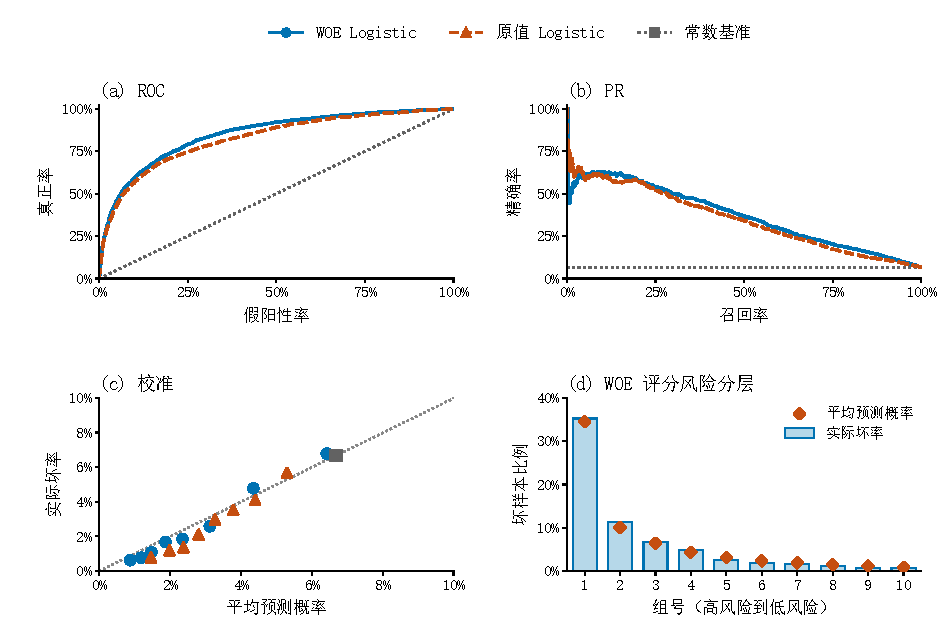
\includegraphics[width=\linewidth,trim=6bp 145bp 1bp 3bp,clip]{figures/test_evaluation.pdf}
  \caption{三模型的 ROC 与 PR 曲线}
  \label{fig:evaluation-roc-pr}
\end{figure}

图~\ref{fig:evaluation-roc-pr}(b) 以召回率为横轴，精确率 $\mathrm{TP}/(\mathrm{TP}+\mathrm{FP})$ 为纵轴，
展示随阈值变化的坏样本覆盖程度与标记对象中坏样本的占比。
记阈值由高到低变化时的召回率与精确率为 $R_j,P_j$，则
$\mathrm{AP}=\sum_j(R_j-R_{j-1})P_j$，按新增召回量加权，召回量不变的点权重为零。
WOE 模型的 AP 为 0.3681，原值模型为 0.3484，常数基准的 AP 等于测试坏样本率 0.0668。
WOE 模型的 AP 约为该基准的 5.51 倍。图中的 PR 水平虚线即测试坏样本率。

测试集坏样本仅占 6.68\%。常数基准在 $t=0.5$ 时漏掉全部坏样本（即坏样本召回率为0漏掉全部坏样本），准确率仍有 93.32\%。
沿图~\ref{fig:evaluation-roc-pr}(b) 的 WOE 曲线从 $t=0.5$ 下调阈值，召回率由 18.15\% 升至 50.02\%，
检出由 364 条增至 1,003 条，误报由 244 条增至 1,722 条。新增误报多于新增检出，总体准确率由 93.72\% 降至 90.92\%。
精确率（precision）则从 59.87\%（364/608）降至 36.81\%（1,003/2,725）。

表~\ref{tab:evaluation-recall-example} 取两模型召回率首次达到 50\% 的曲线点。
同样检出 1,003 条坏样本时，WOE 模型少误报 219 条好样本，精确率由原值模型的 34.07\% 提高至 36.81\%。

\begin{table}[!htbp]
  \centering
  \caption{召回率约 50\% 时的坏样本检出对照}
  \label{tab:evaluation-recall-example}
  \small
  \begin{tabular}{lrrrrr}
    \toprule
    模型 & 检出坏样本 & 误报好样本 & 标记总人数 & 召回率 & 精确率 \\
    \midrule
    WOE Logistic & 1,003 & 1,722 & 2,725 & 50.02\% & 36.81\% \\
    原值 Logistic & 1,003 & 1,941 & 2,944 & 50.02\% & 34.07\% \\
    \bottomrule
  \end{tabular}
\end{table}

\FloatBarrier
下一模块将在验证集上，按误报与漏报代价选择风险标记阈值，按坏样本率上限与最低接受比例选择模拟接受门槛。
冻结后再用测试集评价，说明业务目标如何决定复核或接受范围。

\subsection{概率损失与校准表现}
令 $y_i\in\{0,1\}$ 为实际标签。Brier 分数度量概率的平方误差，对数损失会加重对自信但错误的预测的惩罚。
\[
  \mathrm{Brier}=\frac{1}{n}\sum_{i=1}^n(\widehat p_i-y_i)^2,\qquad
  \mathrm{LogLoss}=-\frac{1}{n}\sum_{i=1}^n
  \bigl[y_i\ln\widehat p_i+(1-y_i)\ln(1-\widehat p_i)\bigr].
\]

与原值模型相比，WOE 模型的 Brier 分数由 0.05226 降至 0.05073，对数损失由 0.19481 降至 0.18599，
相对下降 2.91\% 和 4.53\%。常数基准的两项损失均最高。
概率损失综合反映逐户预测误差，校准图进一步显示哪些风险组的平均预测偏高或偏低。


\begin{figure}[!htbp]
  \centering
  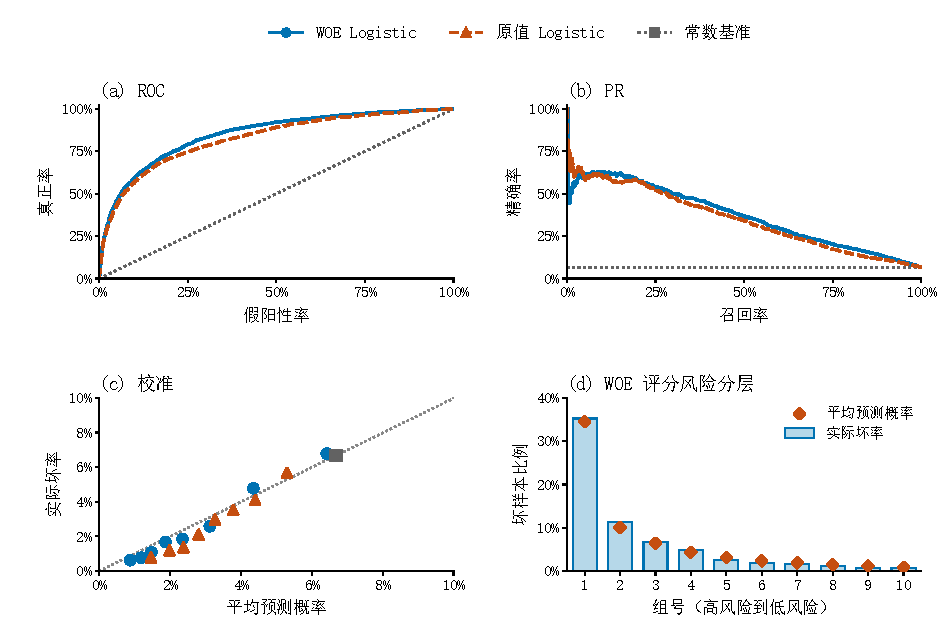
\includegraphics[width=0.66\linewidth,trim=14bp 5bp 222bp 174bp,clip]{figures/test_evaluation.pdf}
  \caption{三模型的测试集校准图（0--10\% 局部放大）}
  \label{fig:evaluation-calibration}

  \smallskip
  \parbox{0.91\linewidth}{\small 注：蓝色圆点为 WOE Logistic，橙色三角为原值 Logistic，灰色方点为常数基准。}
\end{figure}

两个 Logistic 模型分别按各自的预测风险降序分为十组，边界取最接近目标十分位的同值块末尾。
同一预测值的记录归入同组，故 WOE 各组人数介于 2,968 与 3,040，
原值模型恰好每组 3,000 人。设第 $g$ 组有 $n_g$ 人，比较平均预测概率 $\bar p_g$ 与实测坏率
$\bar y_g$。图~\ref{fig:evaluation-calibration} 的对角线表示两者相等，点在线上方表示该组风险被低估。
测试集中，WOE 和原值 Logistic 的逐户预测概率不超过 10\% 的比例分别为 85.77\% 和 87.87\%，
因此图中两轴均放大至 0--10\%。两个模型各有八组的平均预测概率和实际坏率同时落在该区间。
表~\ref{tab:evaluation-calibration} 列出每组人数和偏差，两模型的同序号组各自按预测风险划分。

\begin{table}[H]
  \centering
  \caption{两个 Logistic 模型的分组校准明细}
  \label{tab:evaluation-calibration}
  \small
  \begin{tabular}{c rrrr rrrr}
\toprule
& \multicolumn{4}{c}{WOE Logistic} & \multicolumn{4}{c}{原值 Logistic} \\
\cmidrule(lr){2-5}\cmidrule(lr){6-9}
组 & 人数 & 平均预测 & 实际坏率 & 差值 & 人数 & 平均预测 & 实际坏率 & 差值 \\
\midrule
1 & 3,001 & 34.50\% & 35.25\% & $+0.75$ & 3,000 & 32.48\% & 33.80\% & $+1.32$ \\
2 & 3,010 & 10.07\% & 11.43\% & $+1.36$ & 3,000 & 8.33\% & 11.33\% & $+3.01$ \\
3 & 2,992 & 6.42\% & 6.78\% & $+0.36$ & 3,000 & 5.30\% & 5.67\% & $+0.37$ \\
4 & 2,992 & 4.35\% & 4.78\% & $+0.43$ & 3,000 & 4.40\% & 4.10\% & $-0.30$ \\
5 & 2,980 & 3.12\% & 2.58\% & $-0.54$ & 3,000 & 3.78\% & 3.53\% & $-0.25$ \\
6 & 3,029 & 2.35\% & 1.85\% & $-0.50$ & 3,000 & 3.27\% & 2.97\% & $-0.30$ \\
7 & 2,992 & 1.87\% & 1.67\% & $-0.20$ & 3,000 & 2.81\% & 2.10\% & $-0.71$ \\
8 & 2,968 & 1.47\% & 1.08\% & $-0.40$ & 3,000 & 2.38\% & 1.37\% & $-1.01$ \\
9 & 2,996 & 1.19\% & 0.77\% & $-0.42$ & 3,000 & 1.98\% & 1.20\% & $-0.78$ \\
10 & 3,040 & 0.88\% & 0.62\% & $-0.25$ & 3,000 & 1.46\% & 0.77\% & $-0.70$ \\
\bottomrule
\end{tabular}


  \smallskip
  \parbox{0.94\linewidth}{\small 注：差值为实际坏率减平均预测概率，单位为百分点。常数基准单列一组，共 30,000 人，平均预测为 6.6844\%，实际坏率为 6.6833\%。}
\end{table}

WOE 模型前四组的平均预测低于实际坏率，后六组则偏高。偏差最明显的是第 2 组，
预测为 10.07\%，实际为 11.43\%。原值模型同序号组的预测为 8.33\%，
实际为 11.33\%。按人数加权的绝对组差
$\sum_g(n_g/n)|\bar y_g-\bar p_g|$ 在 WOE 模型为 0.52\%，在原值模型为 0.87\%。
这一统计量依赖分组方式。


\subsection{WOE 评分的风险分层}
按式~\eqref{eq:score-probability}，未取整总分越低，预测坏样本概率越高。
将测试记录按未取整分数升序排列，沿用上述近似等频方法划分十组，保留每个同分块的完整性。
第 1 组是最低分、最高风险组。表~\ref{tab:evaluation-risk-groups} 列出各组观测分数范围、人数、
坏样本数、平均预测和实际坏率。第 $g$ 组的累计覆盖率为前 $g$ 组坏样本数之和除以全部 2,005 条坏样本。

\begin{table}[H]
  \centering
  \caption{WOE 评分的十组风险分层}
  \label{tab:evaluation-risk-groups}
  \small
  \setlength{\tabcolsep}{6pt}
  \begin{tabular}{rrrrrrr}
\toprule
组 & 观测分数范围 & 人数 & 坏样本 & 平均预测 & 实际坏率 & 累计覆盖 \\
\midrule
1 & 434.095--566.542 & 3,001 & 1,058 & 34.50\% & 35.25\% & 52.77\% \\
2 & 566.579--585.813 & 3,010 & 344 & 10.07\% & 11.43\% & 69.93\% \\
3 & 585.815--598.843 & 2,992 & 203 & 6.42\% & 6.78\% & 80.05\% \\
4 & 598.849--610.015 & 2,992 & 143 & 4.35\% & 4.78\% & 87.18\% \\
5 & 610.102--618.179 & 2,980 & 77 & 3.12\% & 2.58\% & 91.02\% \\
6 & 618.193--626.538 & 3,029 & 56 & 2.35\% & 1.85\% & 93.82\% \\
7 & 626.591--632.496 & 2,992 & 50 & 1.87\% & 1.67\% & 96.31\% \\
8 & 632.615--639.667 & 2,968 & 32 & 1.47\% & 1.08\% & 97.91\% \\
9 & 639.830--647.650 & 2,996 & 23 & 1.19\% & 0.77\% & 99.05\% \\
10 & 647.982--663.133 & 3,040 & 19 & 0.88\% & 0.62\% & 100.00\% \\
\bottomrule
\end{tabular}


  \smallskip
  \parbox{0.94\linewidth}{\small 注：分数范围为本组样本的实际最小值至最大值，按三位小数展示。组别由高风险排至低风险。}
\end{table}

\begin{figure}[H]
  \centering
  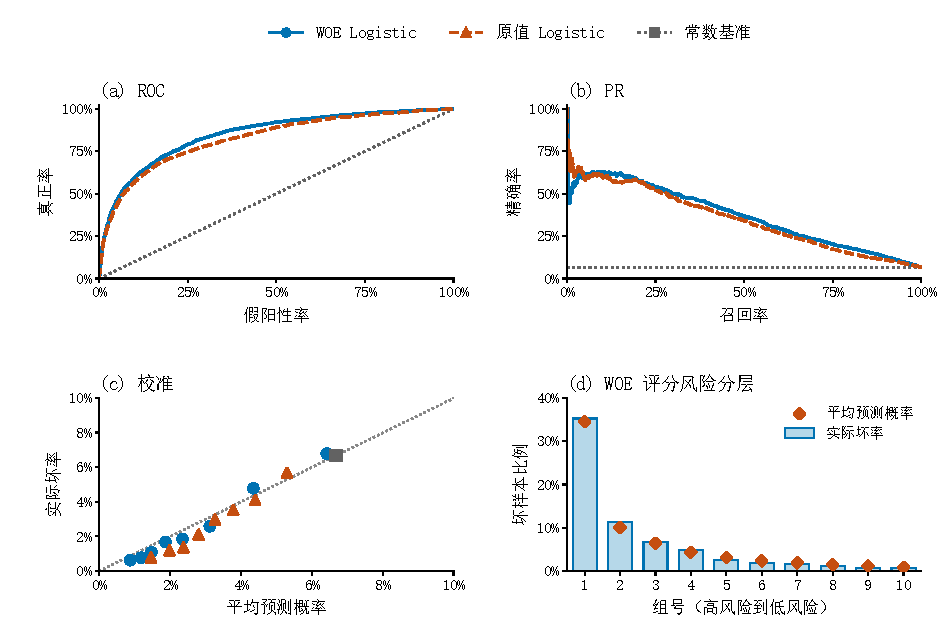
\includegraphics[width=0.66\linewidth,trim=238bp 5bp 4bp 174bp,clip]{figures/test_evaluation.pdf}
  \caption{WOE 评分各组的平均预测与实际坏率}
  \label{fig:evaluation-risk-groups}
\end{figure}

图~\ref{fig:evaluation-risk-groups} 显示，实际坏率随分数提高逐组下降。
第 1 组坏率为 35.25\%，约为总体坏率的 5.28 倍。第 2 组降至 11.43\%，第 3 组为 6.78\%，接近总体水平。
最低风险组 3,040 人中有 19 条坏样本，坏率为 0.625\%。这一结果表明评分在测试集中形成了可观察的风险梯度。

按风险从高到低检查客户时，先覆盖第 1 组约 10.00\% 的记录，就能覆盖 1,058 条坏样本，
占全部坏样本的 52.77\%。覆盖前两组约 20.04\% 的记录时，累计覆盖率提高到 69.93\%。
再纳入第 3 组，覆盖 9,003 人（30.01\%）和 1,605 条坏样本（80.05\%）。
边际检出率随检查范围扩大而降低，例如第 3 组每百人约检出 7 条坏样本，低于第 1 组的约 35 条。
这些比例描述测试集上的风险集中程度，供后续分析处理容量与检出量的取舍。
